\subsection{Ensamblado del prototipo}

En la figura~\figref{fig:prototype1} y la figura figura~\figref{fig:prototype2} puede verse como se ensambló el prototipo para facilitar las mediciones a realizar, se utilizaron borneras para facilitar el conexionado de las fuentes de alimentación, la carga y las masas de los instrumentos de medición, de las borneras se tomaron cables con conectores tipo \textit{plug} macho, para la conexión al prototipo que usa los conectores \textit{plug} hembra, asegurando una buena conexión. Finalmente todo el conjunto usando pilares metálicos para la placa del amplificador, se montó sobre una madera que sostiene el conjunto y permite moverlo y transportarlo fácilmente.

\begin{figure}[H]
    \centering
    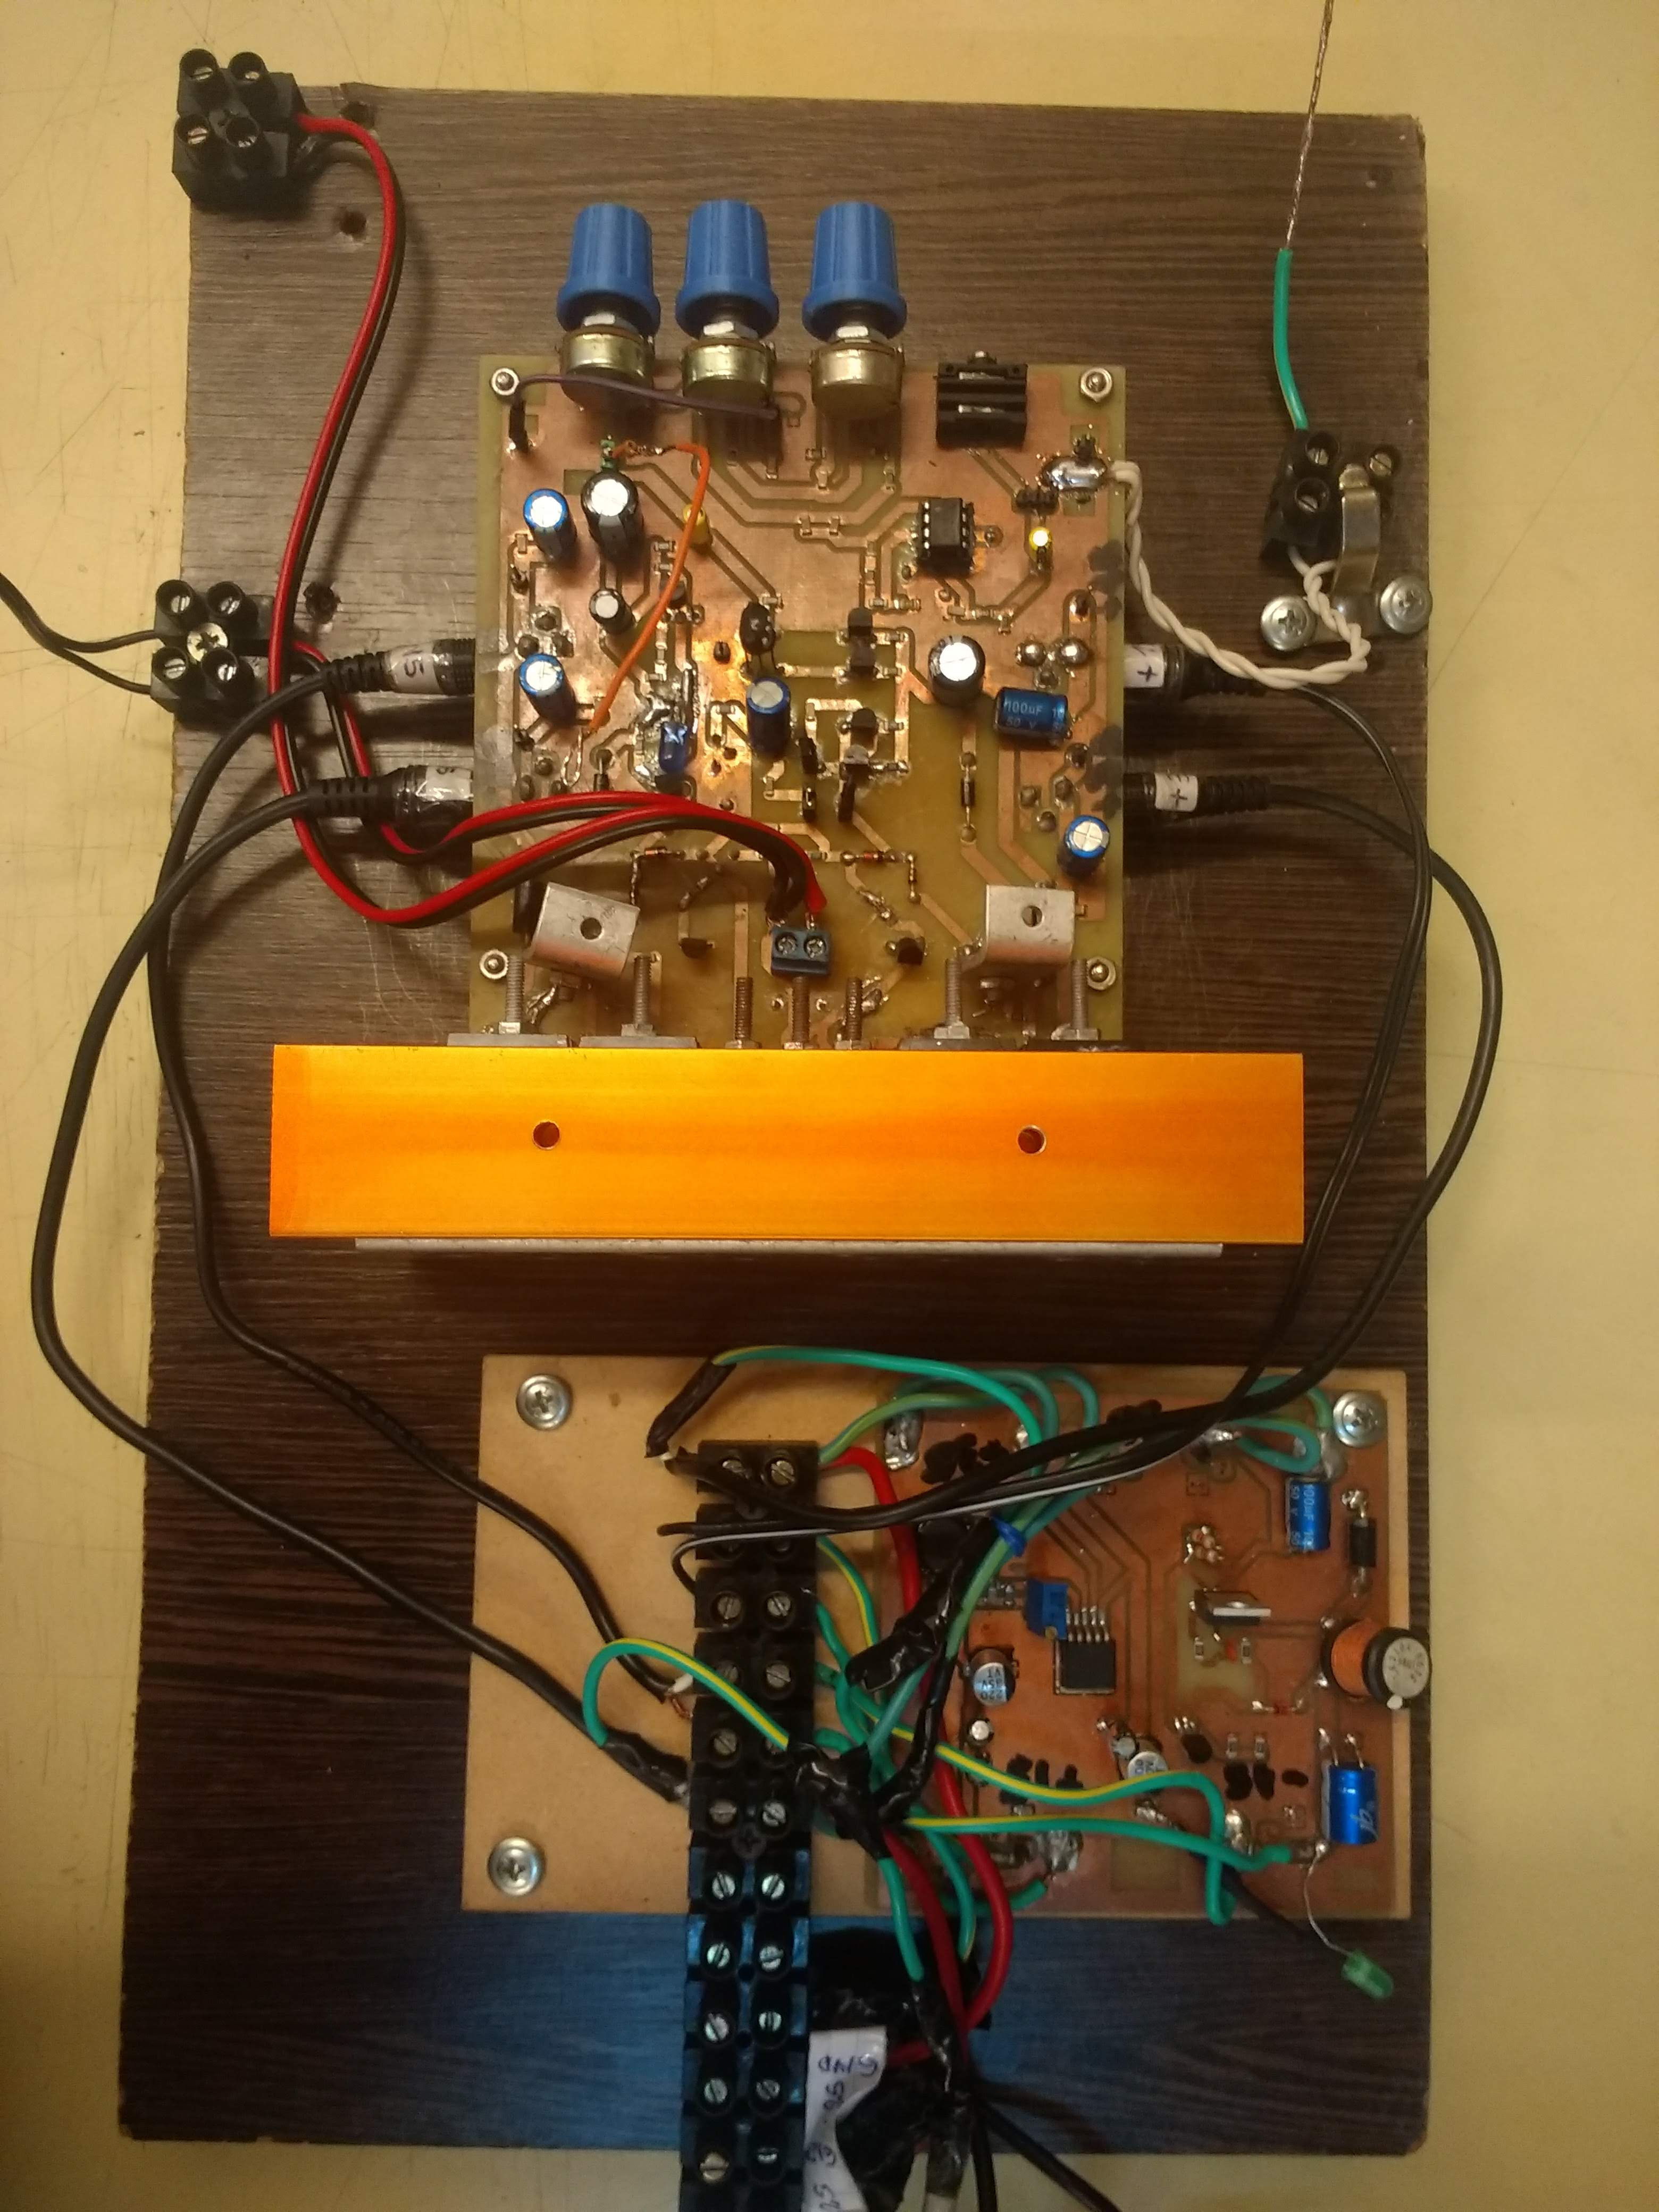
\includegraphics[height=0.95 \textwidth, angle=90]{img/fotos/8.jpg}
    \caption{Ensamblado del prototipo.}
    \label{fig:prototype1}
\end{figure}


\vfill

\clearpage


\begin{figure}[H]
    \centering
    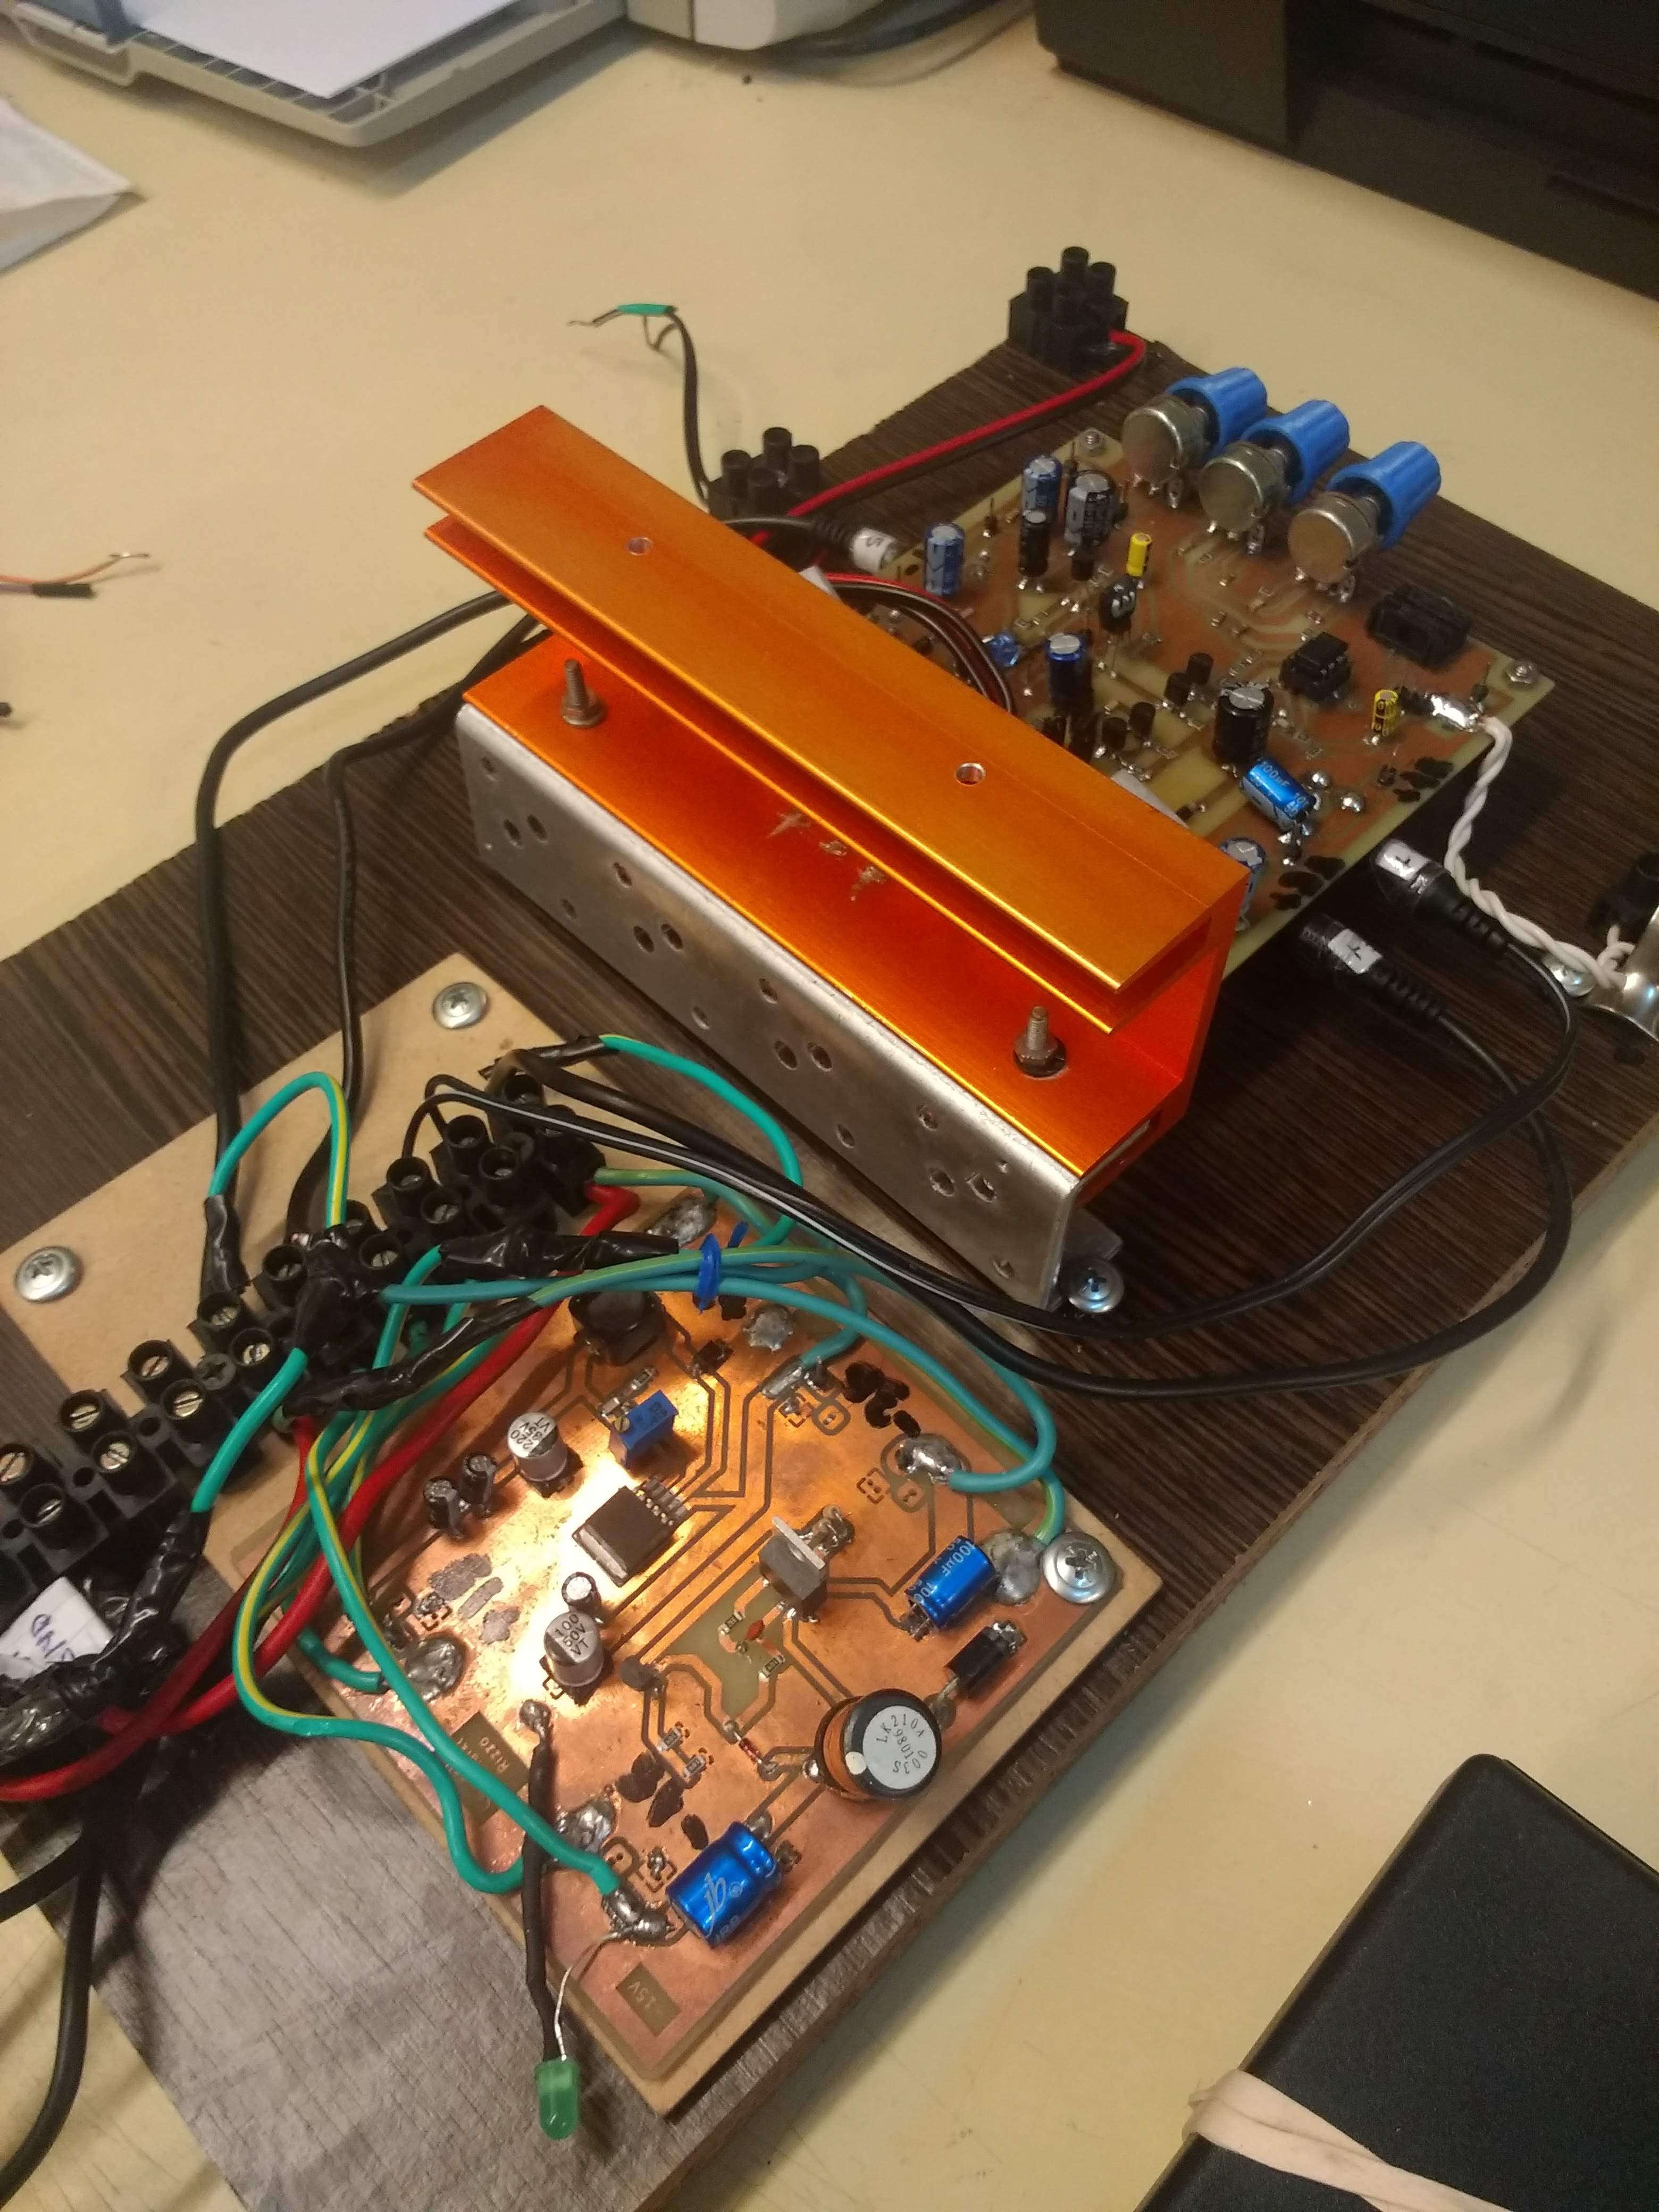
\includegraphics[height=0.95 \textwidth, angle=0]{img/fotos/2.jpg}
    \caption{Detalle del amplificador.}
    \label{fig:prototype2}
\end{figure}


\vfill

\clearpage


En la figura~\figref{fig:prototype2} y la figura~\figref{fig:prototype3}, pueden verse el detalle del amplificador y de la fuente de alimentación interna respectivamente.


\begin{figure}[H]
    \centering
    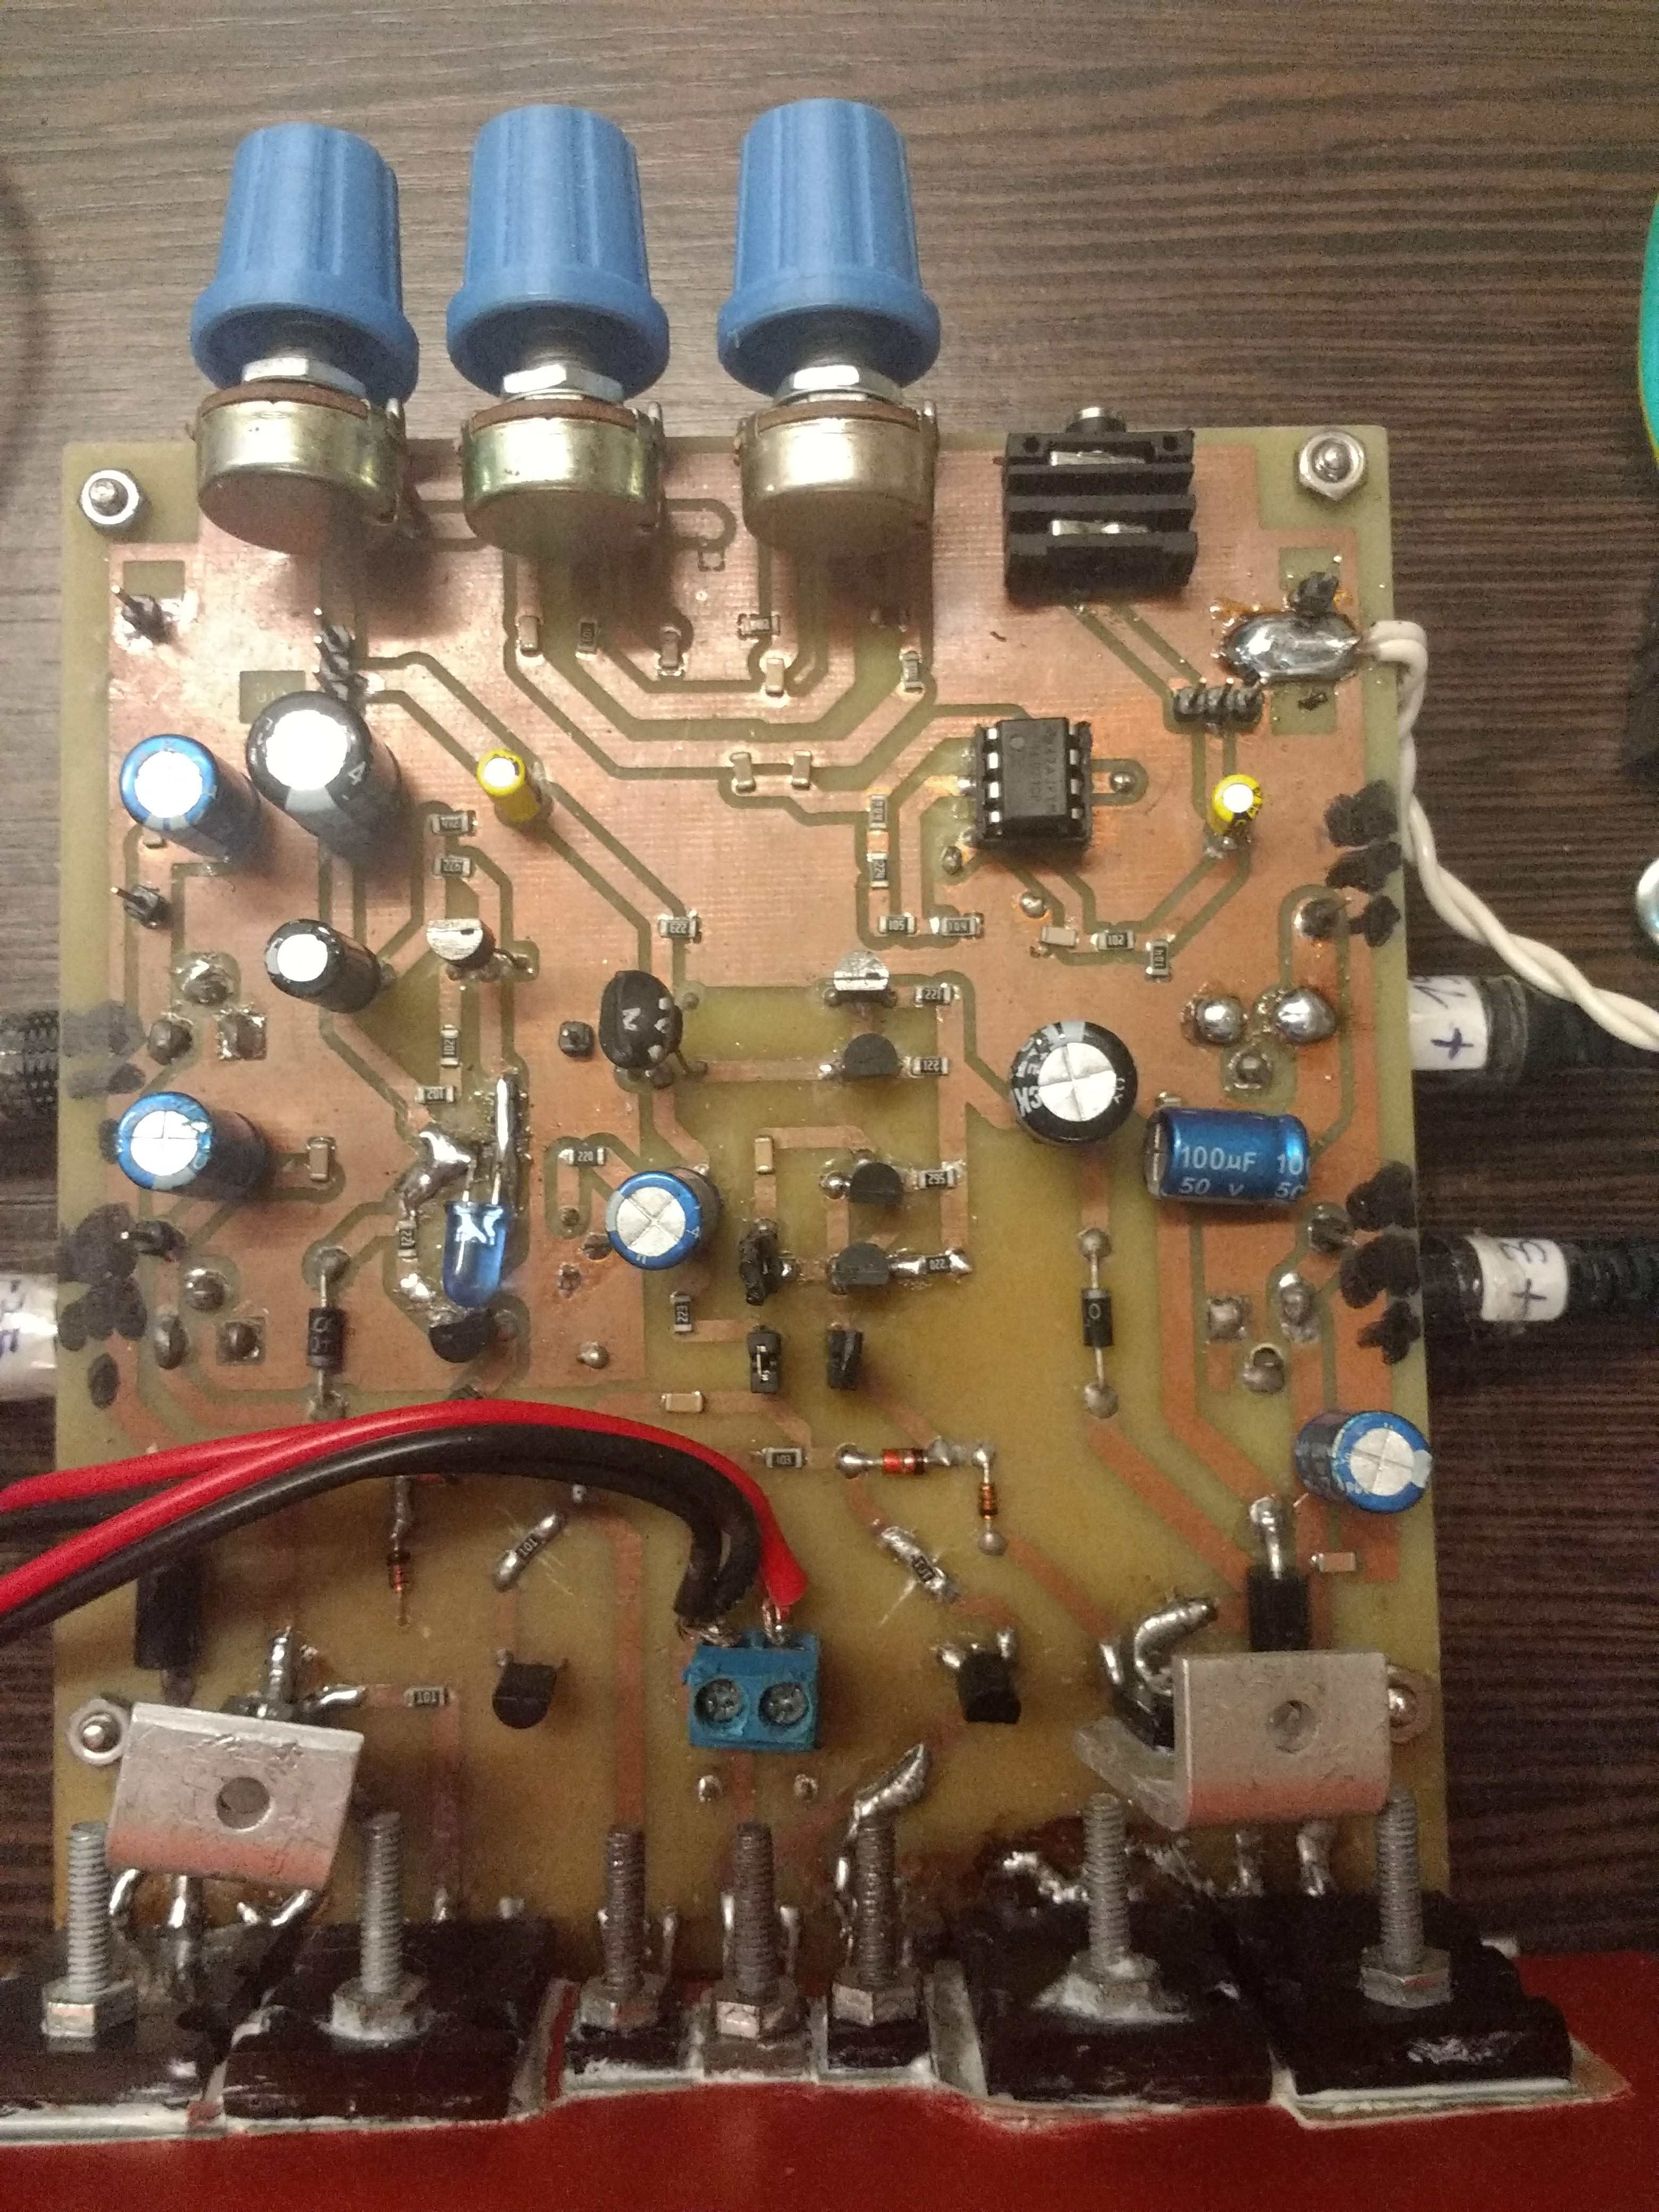
\includegraphics[height=0.7 \textwidth, angle=90]{img/fotos/1.jpg}
    \caption{Detalle del amplificador.}
    \label{fig:prototype3}
\end{figure}

\begin{figure}[H]
    \centering
    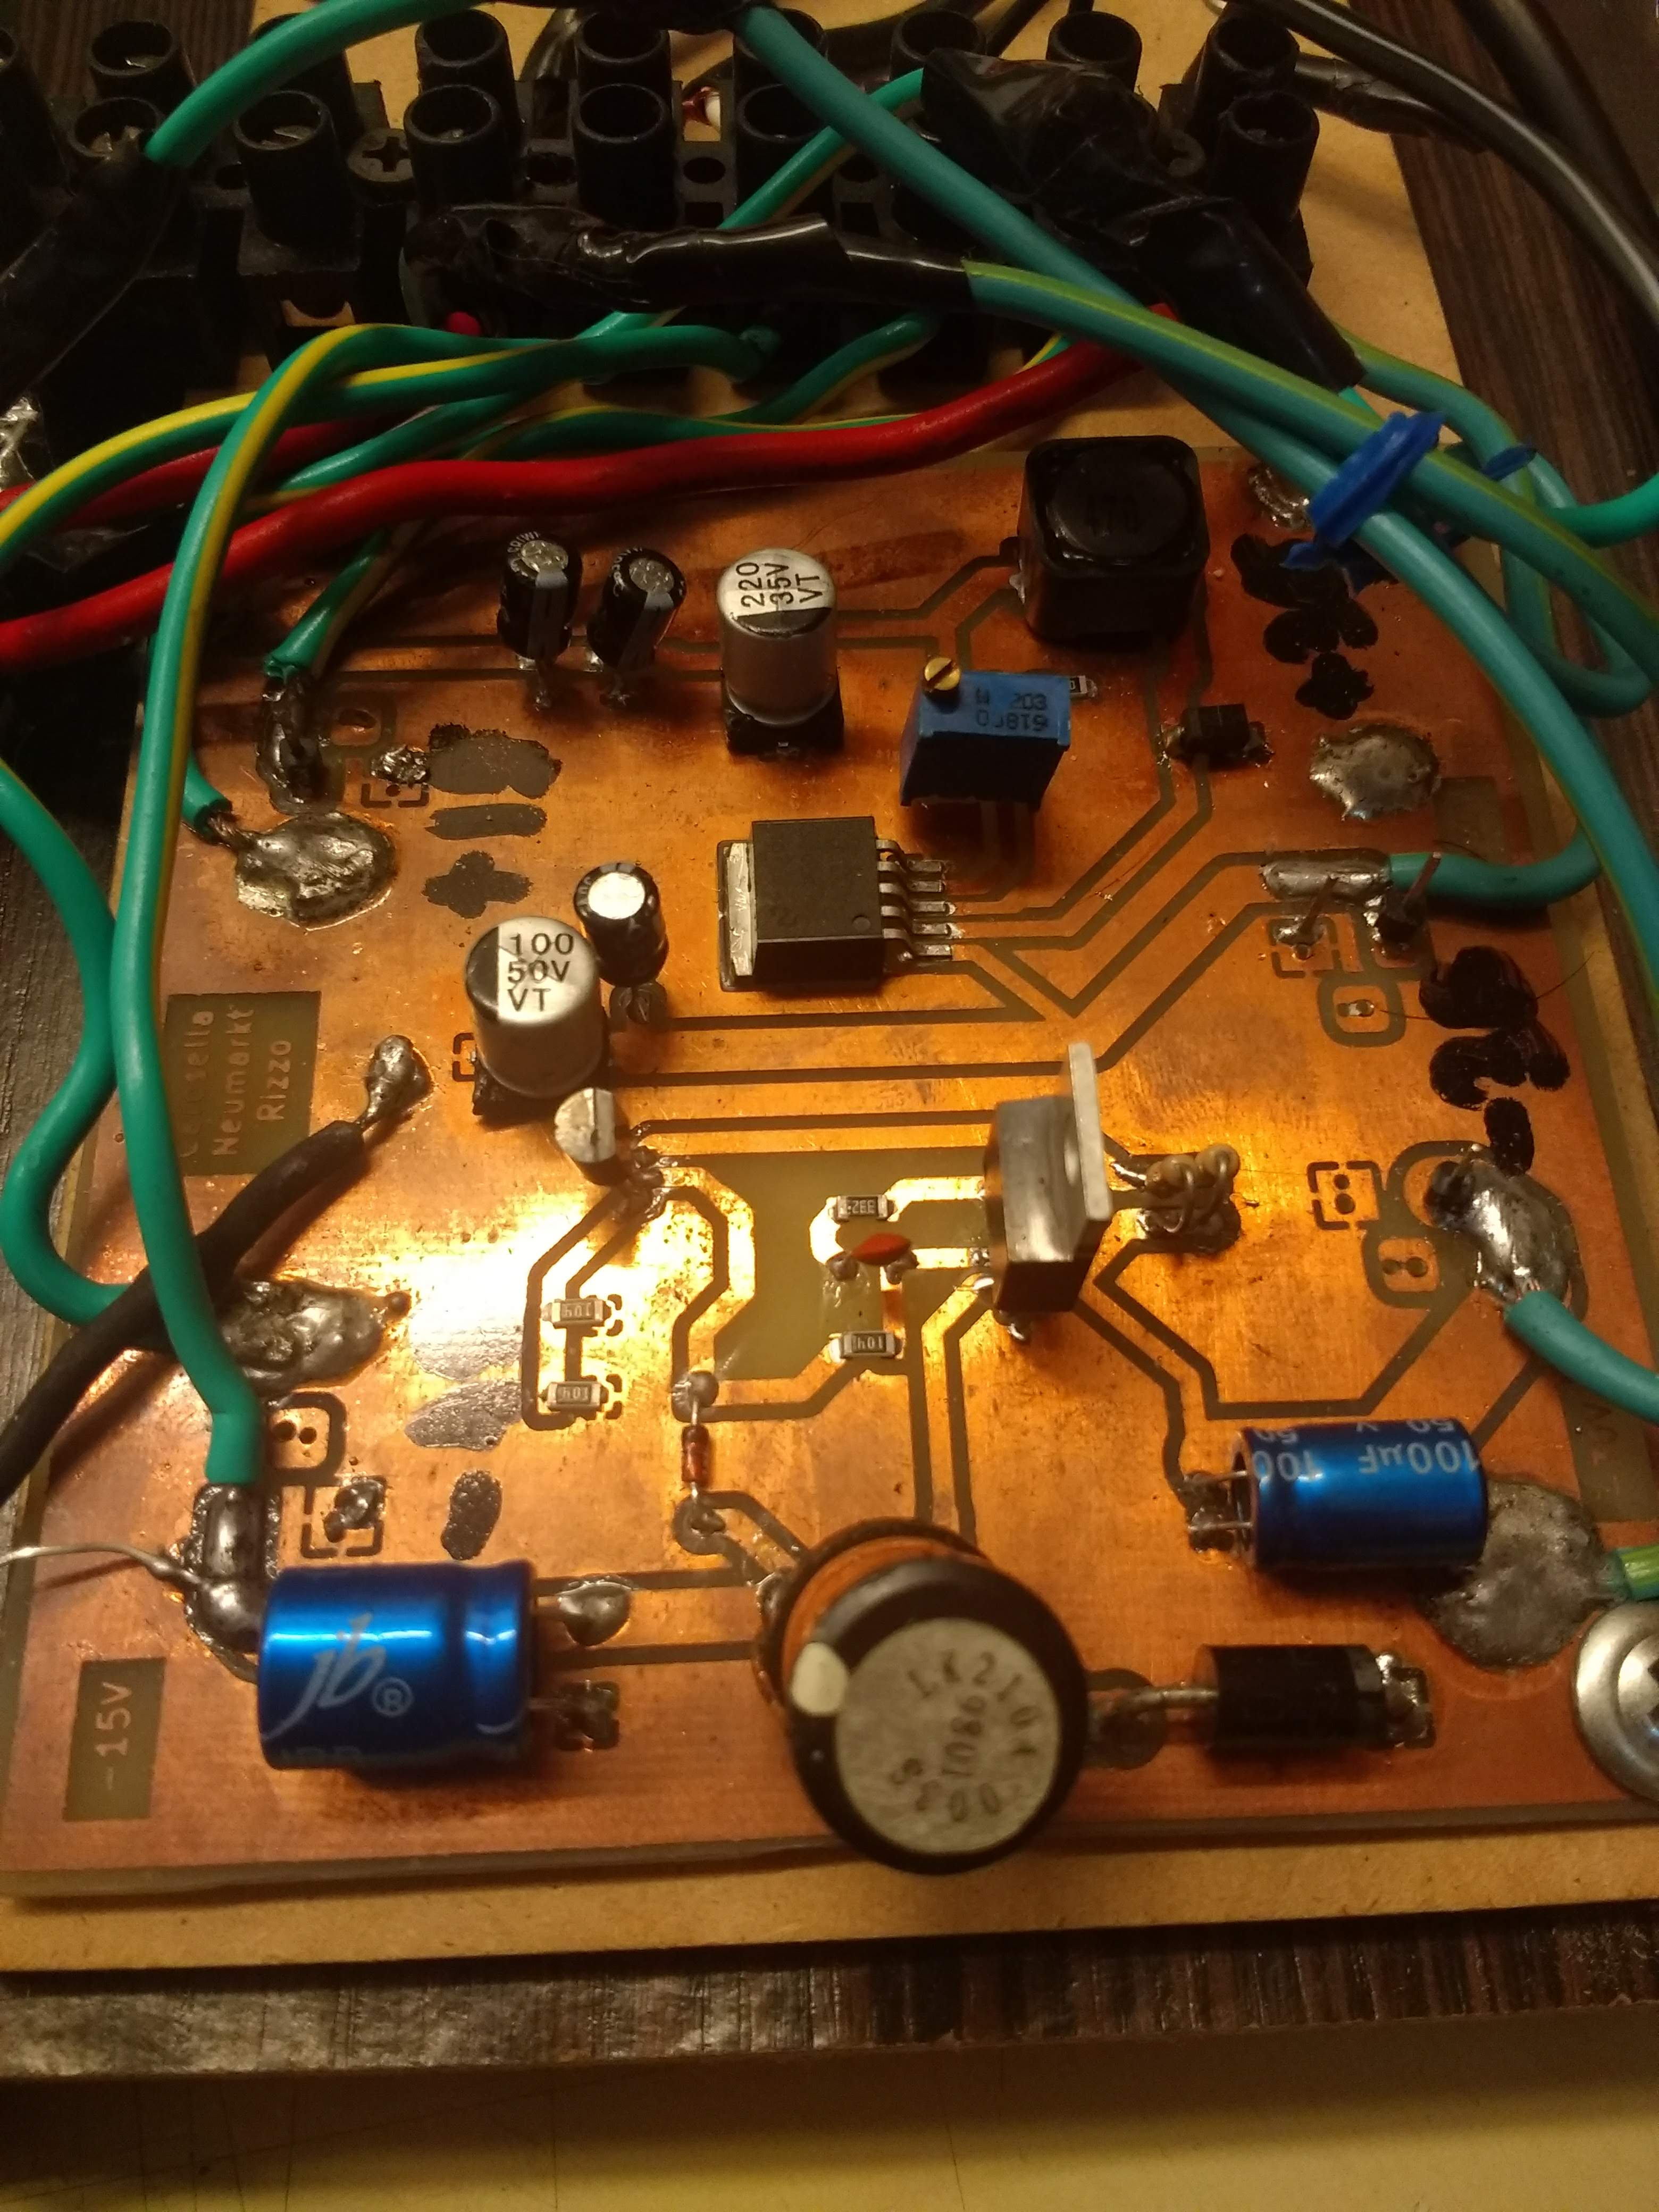
\includegraphics[height=0.7 \textwidth, angle=90]{img/fotos/4.jpg}
    \caption{Detalle de la fuente de alimentación interna.}
    \label{fig:prototype4}
\end{figure}